%
% teil3.tex -- Beispiel-File für Teil 3
%
% (c) 2020 Prof Dr Andreas Müller, Hochschule Rapperswil
%

%
% Modulationsarten
%
\section{Modulationsarten
\label{fm:section:modulation}}
\kopfrechts{Modulationsarten}
Durch die Modulation wird ein Nachrichtensignal \(m(t)\) so mit einem
Trägersignal (z.B.~ein Sinus- oder Rechtecksignal) kombiniert,
dass es übertragen und später wieder decodiert werden kann.
Modulation ist nötig, weil die Frequenzen des Nachrichtensignals
nicht direkt übertragen werden können.
Die Modulation bringt sie in den gewünschten Frequenzbereich, in dem
eine Übertragung möglich ist.

Der ursprünglich Frequenzbereich des Nachrichtensignals \(m(t)\)
erstreckt sich typischerweise von 0 Hz bis zur Bandbreite \(B_m\).
Beim Empfänger wird dann durch Demodulation das ursprüngliche
Nachrichtensignal \(m(t)\) so originalgetreu wie möglich zurückgewonnen.
Beim Trägersignal \(x_c(t)\) handelt es sich um ein informationsloses
Hilfssignal.
Durch die Modulation mit dem Nachrichtensignal \(m(t)\) wird es zum
modulierten Signal für die Übertragung.
Für alle nachfolgenden Erklärungen wird ein sinusförmiges Trägersignal
benutzt, jedoch kann auch ein Rechtecksignal, welches Digital einfach
umzusetzten ist, genauso als Trägersignal genutzt werden \cite{fm:NAT}.

\subsection{Mathematische Beschreibung}
Wir schreiben
das sinusförmige Trägersignal im Folgenden in der Form
\[
x_c(t) = A_c \cdot \cos(\omega_c(t)+\varphi).
\]
Darin kann die Amplitude \(A_c\) und Phase \(\varphi\) des
Nachrichtensignals \(m(t)\) verändert werden.
Der Parameter \(\omega_c\), die Trägerkreisfrequenz, bzw.~die
Trägerfrequenz \(f_c = \frac{\omega_c}{2\pi}\)
steht nicht für die Modulation zur Verfügung, statt dessen kann durch
ihn die Frequenzachse frei gewählt werden.
Dies ist für die Vielfalt der Modulationsarten keine Einschränkung.

Ein Nachrichtensignal kann auch über die Momentanfrequenz
\(\omega_i\)
(engl.: instantenous frequency)
eines Trägers charakterisiert werden.
Mathematisch wird dann daraus
\[
    \omega_i = \omega_c + \frac{d \varphi(t)}{dt}
\]
mit der Ableitung der Phase\cite{fm:NAT}.

Mit diesen drei Parameter ergeben sich auch drei Modulationsarten,
die Amplitudenmodulation, welche \(A_c\) in Abb.~\ref{fig:fm:AM} benutzt, 
die Phasenmodulation \(\varphi\) in Abb.~\ref{fig:fm:PM} und dann noch
eine Modulation, die Momentankreisfrequenz \(\omega_i\) wie in
Abb.~\ref{fig:fm:FM} manipuliert.
Am anschaulichsten und einfachsten zu verstehen ist die
Amplitudenmodulation.

\begin{figure}
    \centering
	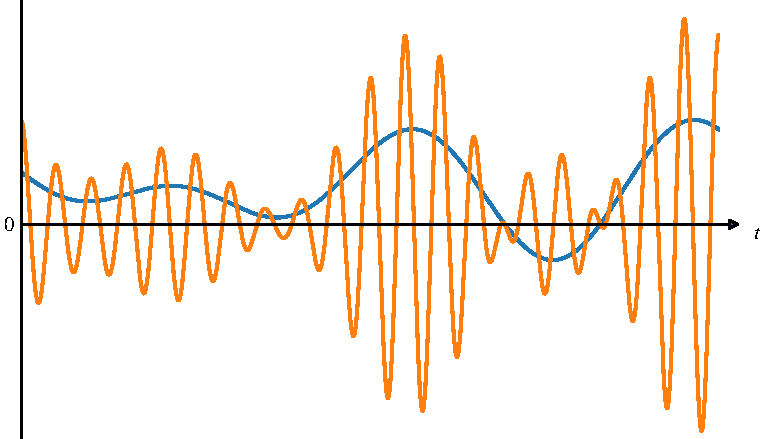
\includegraphics{papers/fm/images/am.pdf}
	\caption{Modulationsart Amplitudenmodulation mit dem Parameter \(A_c\)}
	\label{fig:fm:AM}
\end{figure}

\begin{figure}
    \centering
	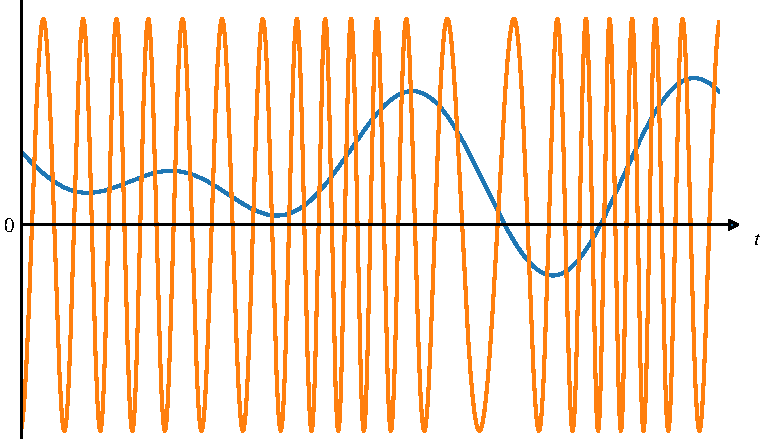
\includegraphics{papers/fm/images/pm.pdf}
	\caption{Modulationsart Phasenmodulation mit dem Parameter \(\varphi\)}
	\label{fig:fm:PM}
\end{figure}

\begin{figure}
    \centering
	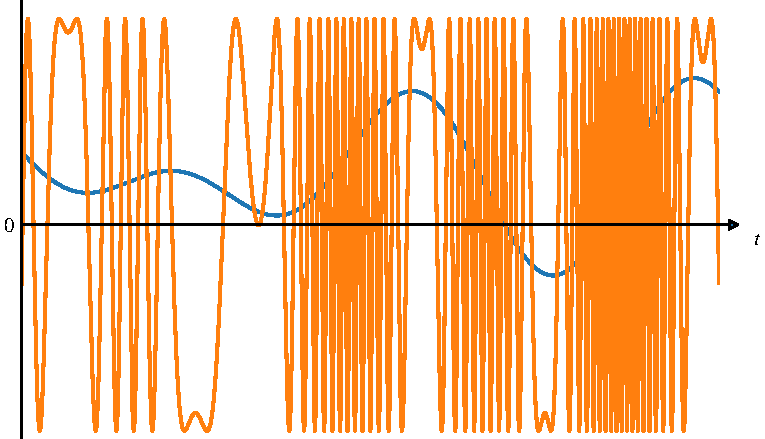
\includegraphics{papers/fm/images/fm.pdf}
	\caption{Modulationsart Freguenzmodulation mit dem Parameter \(\omega_i\)}
	\label{fig:fm:FM}
\end{figure}





